\documentclass[12pt]{article}
\usepackage{amsmath}
\usepackage{graphicx}
\usepackage{hyperref}
\usepackage{listings}
\usepackage{color}

\title{Operating System Course Report - First Half of the Semester}
\author{B class}
\date{\today}

\begin{document}

\maketitle
\newpage

\tableofcontents
\newpage

\section{Introduction}
This report summarizes the topics covered during the first half of the Operating System course. It includes theoretical concepts, practical implementations, and assignments. The course focuses on the fundamentals of operating systems, including system architecture, process management, CPU scheduling, and deadlock handling.

\section{Course Overview}
\subsection{Objectives}
The main objectives of this course are:
\begin{itemize}
    \item To understand the basic components and architecture of a computer system.
    \item To learn process management, scheduling, and inter-process communication.
    \item To explore file systems, input/output management, and virtualization.
    \item To study the prevention and handling of deadlocks in operating systems.
\end{itemize}

\subsection{Course Structure}
The course is divided into two halves. This report focuses on the first half, which covers:
\begin{itemize}
    \item Basic Concepts and Components of Computer Systems
    \item System Performance and Metrics
    \item System Architecture of Computer Systems
    \item Process Description and Control
    \item Scheduling Algorithms
    \item Process Creation and Termination
    \item Introduction to Threads
    \item File Systems
    \item Input and Output Management
    \item Deadlock Introduction and Prevention
    \item User Interface Management
    \item Virtualization in Operating Systems
\end{itemize}

\section{Topics Covered}

\subsection{Basic Concepts and Components of Computer Systems}
This section explains the fundamental components that make up a computer system, including the CPU, memory, storage, and input/output devices.

\subsection{System Performance and Metrics}
This section introduces various system performance metrics used to measure the efficiency of a computer system, including throughput, response time, and utilization.

\subsection{System Architecture of Computer Systems}
Describes the architecture of modern computer systems, focusing on the interaction between hardware and the operating system.

\subsection{Process Description and Control}
Processes are a central concept in operating systems. This section covers:
\begin{itemize}
    \item Process states and state transitions
    \item Process control block (PCB)
    \item Context switching
\end{itemize}

\subsection{Scheduling Algorithms}
This section covers:
\begin{itemize}
    \item First-Come, First-Served (FCFS)
    \item Shortest Job Next (SJN)
    \item Round Robin (RR)
\end{itemize}
It explains how these algorithms are used to allocate CPU time to processes.

\subsection{Process Creation and Termination}
Details how processes are created and terminated by the operating system, including:
\subsubsection{Pembuatan dan Terminasi Proses}
Bagian ini menjelaskan bagaimana proses diakhiri oleh sistem operasi, dengan fokus pada proses terminasi dan pembersihan yang terjadi setelahnya. Proses terminasi adalah tahapan akhir dari siklus hidup proses yang ditangani secara hati-hati oleh sistem operasi untuk mencegah masalah seperti kebocoran memori, penggunaan sumber daya yang tidak efisien, atau penguncian sumber daya. Setelah terminasi, langkah-langkah pembersihan (cleanup) menjadi penting dalam menjaga stabilitas dan kinerja sistem secara keseluruhan.

\subsubsection{Proses Terminasi dan Kondisi Cleanup}
Ketika sebuah proses berakhir, beberapa mekanisme sistem operasi akan melakukan langkah-langkah untuk melepaskan dan mendaur ulang sumber daya yang telah digunakan oleh proses. Proses cleanup ini bertujuan agar sumber daya tersebut dapat digunakan kembali oleh proses lain. Proses terminasi mencakup de-allocating sumber daya yang digunakan, menghapus informasi dari tabel proses, dan mengembalikan status eksekusi ke proses induk.

\subsubsection{De-Alokasi Sumber Daya}
Sumber daya yang digunakan oleh sebuah proses selama masa hidupnya meliputi memori, file, dan perangkat keras. Ketika proses selesai, sumber daya tersebut harus dilepaskan. Jika tidak, sistem akan kehabisan sumber daya yang menyebabkan kinerja sistem menurun. De-allocating atau pelepasan sumber daya ini sangat krusial karena setiap byte memori atau perangkat keras yang tidak dibebaskan dapat membuat sistem menjadi kurang efisien. Berikut penjelasan lebih detail tentang jenis sumber daya yang dilepaskan:

\begin{itemize}
    \item \textbf{Memori (RAM)}: Memori yang dialokasikan ke suatu proses harus dikembalikan ke pool memori setelah proses berakhir. RAM yang tidak dibebaskan kembali ke sistem dapat menyebabkan kebocoran memori (\textit{memory leak}), yaitu kondisi di mana memori yang tidak terpakai tetap terkunci oleh proses yang telah berakhir. Jika kebocoran memori ini dibiarkan, sistem akan mengalami penurunan kinerja karena kapasitas memori yang tersedia semakin berkurang seiring dengan berjalannya waktu, hingga akhirnya menyebabkan sistem melambat atau crash.
    
    \item \textbf{File yang Terbuka}: Ketika sebuah proses membuka file selama eksekusi, file tersebut harus ditutup setelah proses selesai. File descriptor yang tetap terbuka dapat mengunci file tersebut, sehingga tidak dapat diakses oleh proses lain yang memerlukannya. Selain itu, jika jumlah file descriptor yang tidak tertutup meningkat, sistem bisa mencapai batas maksimum file descriptor yang dapat dibuka. Ini menyebabkan aplikasi atau proses baru tidak dapat membuka file karena tidak ada lagi file descriptor yang tersedia, dan ini dapat mengakibatkan kegagalan dalam eksekusi proses lain.
    
    \item \textbf{Perangkat Keras yang Digunakan}: Beberapa proses membutuhkan akses eksklusif ke perangkat keras tertentu, misalnya port jaringan, printer, atau disk drive. Setelah proses berakhir, akses eksklusif ini harus dilepaskan, sehingga perangkat keras tersebut dapat digunakan oleh proses lain. Jika perangkat keras tidak dilepaskan dengan benar, perangkat tersebut bisa tetap terkunci oleh proses yang telah berakhir, menyebabkan masalah bagi proses lain yang mencoba menggunakan perangkat keras yang sama. Ini bisa menghambat operasi lain dalam sistem dan menyebabkan sistem macet atau tidak responsif.
\end{itemize}

\subsubsection{Menghapus Entri dari Tabel Proses}
Setiap proses di dalam sistem dilacak oleh tabel proses (\textit{Process Table}), yang berisi informasi penting mengenai setiap proses yang berjalan. Setelah proses berakhir, entri dalam tabel proses harus dihapus untuk mencegah masalah yang bisa muncul jika PID yang sama digunakan oleh proses baru. Tabel proses berfungsi sebagai "peta" untuk sistem operasi, yang memungkinkan sistem memantau setiap proses yang berjalan dan sumber daya yang sedang digunakan. Penghapusan entri yang tepat sangat penting dalam menjaga efisiensi dan menghindari kebingungan dalam alokasi sumber daya.

\begin{itemize}
    \item \textbf{Status Proses}: Setiap proses memiliki status, seperti sedang berjalan (\textit{running}), ditunda (\textit{suspended}), atau selesai (\textit{terminated}). Ketika proses telah berakhir, statusnya harus diubah menjadi "terminated" dan entri ini perlu dihapus untuk menghindari konflik dengan proses baru yang mungkin menggunakan PID yang sama. Jika tabel proses tidak diperbarui, sistem mungkin akan menganggap bahwa proses yang sudah berakhir masih berjalan, sehingga dapat menyebabkan penggunaan PID yang tidak benar atau tumpang tindih sumber daya.
    
    \item \textbf{PID (Process ID)}: Setiap proses di sistem operasi memiliki identifikasi unik yang disebut PID. Setelah sebuah proses selesai, PID yang digunakan oleh proses tersebut dikembalikan dan dapat digunakan oleh proses lain. Namun, entri di tabel proses harus dihapus terlebih dahulu untuk memastikan bahwa tidak ada informasi yang salah atau usang terkait proses lama yang dapat mengganggu proses baru yang menggunakan PID tersebut. Proses penghapusan ini memastikan bahwa setiap PID yang digunakan tetap unik dan akurat.
    
    \item \textbf{Informasi Sumber Daya}: Selain status dan PID, tabel proses juga menyimpan informasi terkait sumber daya yang sedang digunakan oleh proses, seperti memori, file descriptor, dan perangkat keras. Setelah proses berakhir, informasi ini harus dihapus untuk memastikan bahwa sumber daya tersebut dapat digunakan oleh proses lain. Ini juga membantu menghindari masalah yang terkait dengan sumber daya yang tersisa terkunci atau tidak tersedia untuk proses baru.
\end{itemize}

\subsubsection{Mengembalikan Status Eksekusi ke Parent Process}
Ketika sebuah proses diciptakan, biasanya ada proses induk (\textit{parent process}) yang bertanggung jawab atas proses tersebut. Setelah proses anak (\textit{child process}) selesai, sistem operasi harus mengembalikan informasi mengenai status eksekusi proses anak ke proses induk. Informasi ini meliputi apakah proses anak berhasil atau gagal, dan alasan mengapa proses berakhir. Mekanisme pengembalian status ini penting agar proses induk dapat mengambil tindakan yang sesuai, seperti melanjutkan eksekusi, menangani kesalahan, atau membuat proses baru.

\begin{itemize}
    \item \textbf{\texttt{wait()}}: Panggilan sistem ini digunakan oleh proses induk untuk menunggu hingga proses anak selesai. Saat proses anak berakhir, kode keluaran (\textit{exit code}) dikembalikan ke proses induk. Kode ini menunjukkan hasil akhir dari proses anak, seperti apakah proses berhasil diselesaikan atau ada kesalahan yang terjadi. Berdasarkan kode keluaran ini, proses induk dapat mengambil tindakan yang sesuai, seperti melanjutkan operasi, melakukan rollback, atau mencoba menjalankan kembali proses anak dengan kondisi yang berbeda.

    
    \item \textbf{\texttt{waitpid()}}: 
    
    Panggilan ini adalah variasi dari \texttt{wait()}, di mana proses induk dapat menunggu proses anak tertentu berdasarkan PID-nya. Ini sangat berguna dalam situasi di mana proses induk memiliki lebih dari satu proses anak yang berjalan secara bersamaan. Dengan \texttt{waitpid()}, proses induk dapat memilih proses anak mana yang ingin dia tunggu, memberikan kontrol yang lebih besar atas pengelolaan proses dan memastikan bahwa eksekusi berjalan lebih efisien dan terstruktur.

 
\end{itemize}
\begin{figure}[]
    \centering
    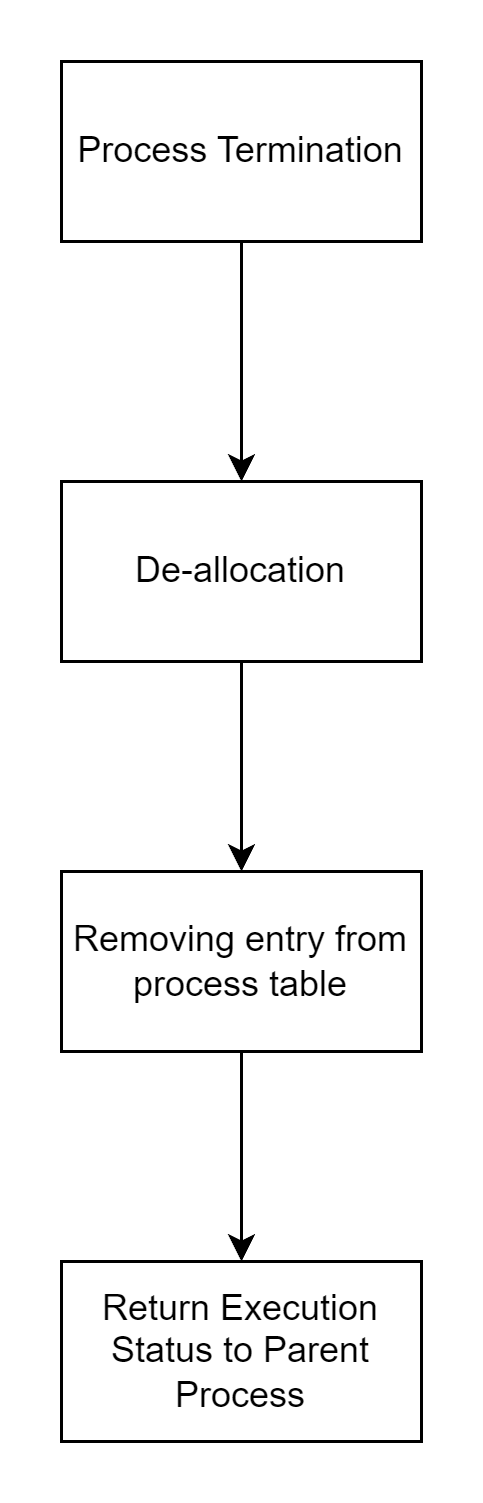
\includegraphics[width=0.2\textwidth]{assets/OSgambar.drawio.png}
    \caption{Diagram alur pembersihan setelah terminasi proses.}
    \label{fig:contoh_gambar}
\end{figure}


\subsection{Introduction to Threads}
This section introduces the concept of threads and their relation to processes, covering:
\begin{itemize}
    \item Single-threaded vs. multi-threaded processes
    \item Benefits of multithreading
\end{itemize}

\subsection{File Systems}
File systems provide a way for the operating system to store, retrieve, and manage data. This section explains:
\begin{itemize}
    \item File system structure
    \item File access methods
    \item Directory management
\end{itemize}

\subsection{Input and Output Management}
Input and output management is key for handling the interaction between the system and external devices. This section includes:
\begin{itemize}
    \item Device drivers
    \item I/O scheduling
\end{itemize}

\subsection{Deadlock Introduction and Prevention}
Explores the concept of deadlocks and methods for preventing them:
\begin{itemize}
    \item Deadlock conditions
    \item Deadlock prevention techniques
\end{itemize}

\subsection{User Interface Management}
This section discusses the role of the operating system in managing the user interface. Topics covered include:
\begin{itemize}
    \item Graphical User Interface (GUI)
    \item Command-Line Interface (CLI)
    \item Interaction between the user and the operating system
\end{itemize}

\subsection{Virtualization in Operating Systems}
Virtualization allows multiple operating systems to run concurrently on a single physical machine. This section explores:

\section{Assignments and Practical Work}
\subsection{Assignment 1: Process Scheduling}
Students were tasked with implementing various process scheduling algorithms (e.g., FCFS, SJN, and RR) and comparing their performance under different conditions.
\subsubsection{Group 1}
\begin{python}
    class Process:
    def __init__(self, pid, arrival_time, burst_time):
        self.pid = pid
        self.arrival_time = arrival_time
        self.burst_time = burst_time
        self.completion_time = 0
        self.turnaround_time = 0
        self.waiting_time = 0
\end{python}

\begin{table}[htbp] % Optional: For floating position
    \centering
    \begin{tabular}{|c|c|c|} % Defines number of columns and alignment (c = center, l = left, r = right). '|' creates vertical lines.
    \hline
    Header 1 & Header 2 & Header 3 \\ % Column headers
    \hline
    Row 1, Column 1 & Row 1, Column 2 & Row 1, Column 3 \\ % First row of data
    \hline
    Row 2, Column 1 & Row 2, Column 2 & Row 2, Column 3 \\ % Second row of data
    \hline
    \end{tabular}
    \caption{Your table caption} % Optional: For adding a caption
    \label{tab:your_label} % Optional: For cross-referencing the table
\end{table}

\subsection{Assignment 2: Deadlock Handling}
In this assignment, students were asked to simulate different deadlock scenarios and explore various prevention methods.

\subsection{Assignment 3: Multithreading and Amdahl's Law}
This assignment involved designing a multithreading scenario to solve a computationally intensive problem. Students then applied **Amdahl's Law** to calculate the theoretical speedup of the program as the number of threads increased.

\subsection{Assignment 4: Simple Command-Line Interface (CLI) for User Interface Management}
Students were tasked with creating a simple **CLI** for user interface management. The CLI should support basic commands such as file manipulation (creating, listing, and deleting files), process management, and system status reporting.

\lstset{
    backgroundcolor=\color{white},   
    basicstyle=\footnotesize\ttfamily,  
    breaklines=true,                
    frame=single,                     
    keywordstyle=\color{blue},      
    commentstyle=\color{green},       
    stringstyle=\color{red},         
}

\begin{document}

\subsection{Assignment 4: Simple Command-Line Interface (CLI) for User Interface Management}
Students were tasked with creating a simple \textbf{CLI} for user interface management. The CLI should support basic commands such as file manipulation (creating, listing, and deleting files), process management, and system status reporting.

\textbf{Deskripsi:} 
Buatlah sebuah program CLI yang dapat melakukan manipulasi file. Program ini harus mampu:
\begin{enumerate}
    \item Membuat file baru dengan nama yang ditentukan oleh pengguna.
    \item Menampilkan daftar semua file yang ada dalam direktori saat ini.
    \item Menghapus file berdasarkan nama yang diberikan oleh pengguna.
\end{enumerate}

\textbf{Kriteria Penilaian:}
\begin{itemize}
    \item Fungsi Pembuat File: Program harus berhasil membuat file dengan nama yang valid.
    \item Fungsi Daftar File: Program harus menampilkan semua file yang ada di direktori saat ini.
    \item Fungsi Penghapusan File: Program harus dapat menghapus file yang ada dan memberikan pesan kesalahan jika file tidak ditemukan.
    \item Antarmuka Pengguna: CLI harus mudah digunakan dan responsif terhadap input pengguna.
\end{itemize}

\paragraph{ANSWER}

\begin{verbatim}
import os
import psutil


def create_file(file_name):
    with open(file_name, 'w') as f:
        f.write('')  # Create an empty file
    print(f"File '{file_name}' created successfully.")

def list_files():
    files = os.listdir()
    if files:
        print("List of files in the current directory:")
        for f in files:
            print(f)
    else:
        print("No files found in the current directory.")


def delete_file(file_name):
    if os.path.exists(file_name):
        os.remove(file_name)
        print(f"File '{file_name}' deleted successfully.")
    else:
        print(f"File '{file_name}' does not exist.")


def list_processes():
    print("List of running processes:")
    for proc in psutil.process_iter(['pid', 'name', 'cpu_percent']):
        print(f"PID: {proc.info['pid']}, Name: {proc.info['name']}, CPU: {proc.info['cpu_percent']}%")

def system_status():
    print("System Status:")
    print(f"CPU usage: {psutil.cpu_percent()}%")
    memory = psutil.virtual_memory()
    print(f"Memory usage: {memory.percent}% ({memory.used / (1024 ** 3):.2f} GB used of {memory.total / (1024 ** 3):.2f} GB)")


def cli():
    while True:
        print("\nSimple CLI Menu:")
        print("1. Create file")
        print("2. List files")
        print("3. Delete file")
        print("4. List processes")
        print("5. System status")
        print("6. Exit")
        
        choice = input("Enter your choice (1-6): ").strip()
        
        if choice == '1':
            file_name = input("Enter the file name to create: ").strip()
            create_file(file_name)
        elif choice == '2':
            list_files()
        elif choice == '3':
            file_name = input("Enter the file name to delete: ").strip()
            delete_file(file_name)
        elif choice == '4':
            list_processes()
        elif choice == '5':
            system_status()
        elif choice == '6':
            print("Exiting CLI...")
            break
        else:
            print("Invalid choice. Please try again.")


if __name__ == "__main__":
    cli()
\end{verbatim}



\subsection{Assignment 5: File System Access}
In this assignment, students implemented file system access routines, including:
\begin{itemize}
    \item File creation and deletion
    \item Reading from and writing to files
    \item Navigating directories and managing file permissions
\end{itemize}

\section{Conclusion}
The first half of the course introduced core operating system concepts, including process management, scheduling, multithreading, and file system access. These topics provided a foundation for more advanced topics to be covered in the second half of the course.

\begin{thebibliography}{}
\bibitem{ref1} Universitas Muhammadiyah Yogyakarta. (n.d.). \textit{Creation and Termination of Processes}. Diambil dari: \url{https://oprek.um.ac.id/proses-spawning}
\bibitem{ref2} University of Illinois Chicago. (n.d.). \textit{Operating System Cleanup After Process Termination}. Diambil dari: \url{https://os-cleanup.uic.edu}
\end{thebibliography}



\end{document}
